\documentclass{ximera}

\newcommand{\RR}{\mathbb R}
\renewcommand{\d}{\,d}
\newcommand{\dd}[2][]{\frac{d #1}{d #2}}
\renewcommand{\l}{\ell}
\newcommand{\ddx}{\frac{d}{dx}}
\newcommand{\dfn}{\textbf}
\newcommand{\eval}[1]{\bigg[ #1 \bigg]}


\author{Jim Talamo}
\license{Creative Commons 3.0 By-bC}


\outcome{Explore the idea that higher order Taylor Polynomials are lower order ones plus correction terms}
\outcome{Introduce an aspect of qualitative reasoning to Taylor polynomials}
\outcome{Show that the quantitative and qualitative approaches are consistent}

\begin{document}
\begin{exercise}
This exercise examines qualitative relationships between a function and its Taylor polynomials and explores how the higher order Taylor polynomials naturally ``correct'' the lower order ones in the context of a specific example.

Consider the function $f(x)=e^{2x}$.  Give the first, second, and third degree Taylor polynomials centered at $x=0$ below:

\begin{align*}
p_1(x) &= \answer{1+2x} \\
p_2(x) &= \answer{1+2x+2x^2} \\
p_3(x) &= \answer{1+2x+2x^2+\frac{4}{3}x^3}
\end{align*}

Note that each higher order polynomial the next lower order one plus a new term.  For instance:

\begin{image}
  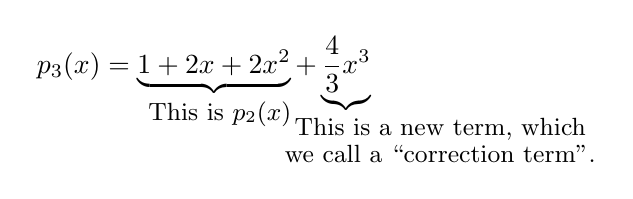
\begin{tikzpicture}
        \node at (0,0) {
          $p_3(x)= \underbrace{1+2x+2x^2}+\underbrace{\frac{4}{3}x^3}$};
        \node at (.2,-.5) {\small{This is $p_2(x)$}}; 
        %%
          \node at (3,-.7) {\small{This is a new term, which}};
          \node at (3,-1) {\small{we call a ``correction term".}};
      \end{tikzpicture}
  \end{image}

This exercise explores what that new ``correction term" does in the context of this specific example.

\begin{exercise}
First, let's look at the graph of $f(x)=e^{2x}$ and $p_1(x)=1+2x$.

\begin{image}
\begin{tikzpicture}

\begin{axis}
	[
	domain=-3:3, ymax=9,xmax=2.3, ymin=-4.5, xmin=-2.3,
	axis lines=center, xlabel=$x$, ylabel=$y$,
	xtick={-2,-1,1,2},
	ytick={-4,-2,2,4,6,8},
	every axis y label/.style={at=(current axis.above origin),anchor=south},
	every axis x label/.style={at=(current axis.right of origin),anchor=west},
	axis on top,
	typeset ticklabels with strut,
	]

	\addplot [draw=penColor,very thick, smooth] {exp(2*x)};
	\addplot [draw=penColor2,very thick, smooth] {1+2*x};
	
	\node at (axis cs:1.7,8) [penColor] {$f(x)=e^{2x}$};
	\node at (axis cs:1.3,1.2) [penColor2] {$p_1(x)=1+2x$};
\end{axis}

\end{tikzpicture}
\end{image}

By looking at the graphs, if we use $p_1(x)$ to approximate $f(x)$ at a nonzero $x$-value $x=x_0$, we expect:
\begin{multipleChoice}
\choice{$p_1(x_0)>f(x_0)$}
\choice[correct]{$p_1(x_0)<f(x_0)$}
\end{multipleChoice}

Indeed, if we pick $x_0 = 1$:

\begin{align*}
f(x_0)=f(1) = e^2 &= \answer[tolerance=.001]{7.389} \textrm{ to $3$ decimal places}\\
p_1(x_0) = p_1(1) &= \answer{3}
\end{align*}

\end{exercise}

\begin{exercise}
Since $p_1(x)$ is always small than $e^{2x}$ when $x \neq 0$, the second degree Taylor polynomial will try to bridge the gap between the lower order polynomial $p_1(x)$ and $e^{2x}$.  

First, note that:

\begin{image}
  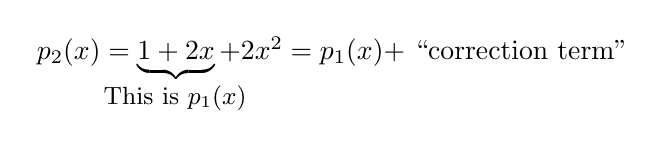
\begin{tikzpicture}
        \node at (0,0) {
          $p_2(x)= \underbrace{1+2x}+2x^2=p_1(x)+$ ``correction term''};
        \node at (-2,-.5) {\small{This is $p_1(x)$}}; 
              \end{tikzpicture}
  \end{image}

Since we established that the first degree Taylor polynomial is an underestimate for the function, this new ``correction term'':

\begin{multipleChoice}
\choice[correct]{should be positive for all $x$.}
\choice{should be positive for $x>0$ and negative for $x<0$.}
\choice{should be negative for $x>0$ and positive for $x<0$.}
\choice{should be negative for all $x$.}
\end{multipleChoice}

Now, from the second degree Taylor polynomial, the actual ``correction term" is $\answer{2x^2}$.  Notice that:
\begin{multipleChoice}
\choice[correct]{$2x^2$ is positive for all $x$.}
\choice{$2x^2$ is  positive for $x>0$ and negative for $x<0$.}
\choice{$2x^2$ is  negative for $x>0$ and positive for $x<0$.}
\choice{$2x^2$ is negative for all $x$.}
\end{multipleChoice}

Does this quantitative result agree with the previous qualitative result that precedes it?
\begin{multipleChoice}
\choice[correct]{Yes}
\choice{No}
\end{multipleChoice}
\end{exercise}

%%%%%%%%%%%%%%%%%
\begin{exercise}
Now, let's look at the graphs of $y=e^{2x}$ and $y=p_2(x)$:

\begin{image}
\begin{tikzpicture}

\begin{axis}
	[
	domain=-3:3, ymax=9,xmax=2.3, ymin=-.5, xmin=-2.3,
	axis lines=center, xlabel=$x$, ylabel=$y$,
	xtick={-2,-1,1,2},
	ytick={-4,-2,2,4,6,8},
	every axis y label/.style={at=(current axis.above origin),anchor=south},
	every axis x label/.style={at=(current axis.right of origin),anchor=west},
	axis on top,
	typeset ticklabels with strut,
	]

	\addplot [draw=penColor,very thick, smooth] {exp(2*x)};
	\addplot [draw=penColor2,very thick, smooth] {1+2*x+2*x^2};
	
	\node at (axis cs:.5,8) [penColor] {$y=e^{2x}$};
	\node at (axis cs:1.6,4) [penColor2] {$y=p_2(x)$};
\end{axis}

\end{tikzpicture}
\end{image}

By simply looking at the graphs above (i.e. WITHOUT examining the third degree polynomial for $e^{2x}$ centered at $x=0$), the ``correction term'' for the third degree Taylor polynomial:

\begin{multipleChoice}
\choice{should be positive for all $x$.}
\choice[correct]{should be positive for $x>0$ and negative for $x<0$.}
\choice{should be negative for $x>0$ and positive for $x<0$.}
\choice{should be negative for all $x$.}
\end{multipleChoice}

Now, from the third degree Taylor polynomial, the actual correction term is $\answer{\frac{4}{3}x^3}$.  Notice that this ``correction term'':
\begin{multipleChoice}
\choice{is positive for all $x$.}
\choice[correct]{is  positive for $x>0$ and negative for $x<0$.}
\choice{is  negative for $x>0$ and positive for $x<0$.}
\choice{ is negative for all $x$.}
\end{multipleChoice}

Does this quantitative result agree with the previous qualitative result that precedes it?
\begin{multipleChoice}
\choice[correct]{Yes}
\choice{No}
\end{multipleChoice}

%%%%%%%%%%%%%%%%%
\begin{exercise}
Now, let's look at the graphs of $y=e^{2x}$ and $y=p_3(x)$:

\begin{image}
\begin{tikzpicture}

\begin{axis}
	[
	domain=-3:3, ymax=9,xmax=2.3, ymin=-4.5, xmin=-2.3,
	axis lines=center, xlabel=$x$, ylabel=$y$,
	xtick={-2,-1,1,2},
	ytick={-4,-2,2,4,6,8},
	every axis y label/.style={at=(current axis.above origin),anchor=south},
	every axis x label/.style={at=(current axis.right of origin),anchor=west},
	axis on top,
	typeset ticklabels with strut,
	]

	\addplot [draw=penColor,very thick, smooth] {exp(2*x)};
	\addplot [draw=penColor2,very thick, smooth] {1+2*x+2*x^2+4/3*x^3};
	
	\node at (axis cs:.5,8) [penColor] {$y=e^{2x}$};
	\node at (axis cs:1.6,5) [penColor2] {$y=p_3(x)$};
\end{axis}

\end{tikzpicture}
\end{image}

By simply looking at the graphs above (i.e. WITHOUT examining the third degree polynomial for $e^{2x}$ centered at $x=0$), the ``correction term'' for the fourth degree Taylor polynomial:

\begin{multipleChoice}
\choice[correct]{should be positive for all $x$.}
\choice{should be positive for $x>0$ and negative for $x<0$.}
\choice{should be negative for $x>0$ and positive for $x<0$.}
\choice{should be negative for all $x$.}
\end{multipleChoice}

The actual fourth degree Taylor polynomial centered at $x=0$ for $f(x)=e^{2x}$ is:

\[
p_4(x) = 1+2x+2x^2+\frac{4}{3}x^3+\frac{2}{3}x^4
\]

so the actual correction term is $\answer{\frac{2}{3}x^4}$, which:

\begin{multipleChoice}
\choice[correct]{is positive for all $x$.}
\choice{is positive for $x>0$ and negative for $x<0$.}
\choice{is negative for $x>0$ and positive for $x<0$.}
\choice{ is negative for all $x$.}
\end{multipleChoice}

Does this quantitative result agree with the previous qualitative result that precedes it?
\begin{multipleChoice}
\choice[correct]{Yes}
\choice{No}
\end{multipleChoice}

We now make an important observation:

\begin{remark}
Note that each of the Taylor polynomials ``overcorrects'' the previous ones; indeed no higher order Taylor polynomial will agree with $e^{2x}$ for all $x$-values since $e^{2x}$ is not a polynomial.  Thus, each higher order Taylor polynomial will try to ``fix'' the overcorrection from the previous one, with the hope that the discrepancies become smaller as higher order Taylor polynomials are used.
\end{remark}

\end{exercise}
\end{exercise}
\end{exercise}
\end{document}
